\section{Experimental Setup}
\label{sec:experiment}
This section adopts an experimental design consistent with prior research protocols~\cite{chengCanShowWhat2021}, and was reviewed and approved by an IRB.

\begin{figure*}[t]
    \centering
    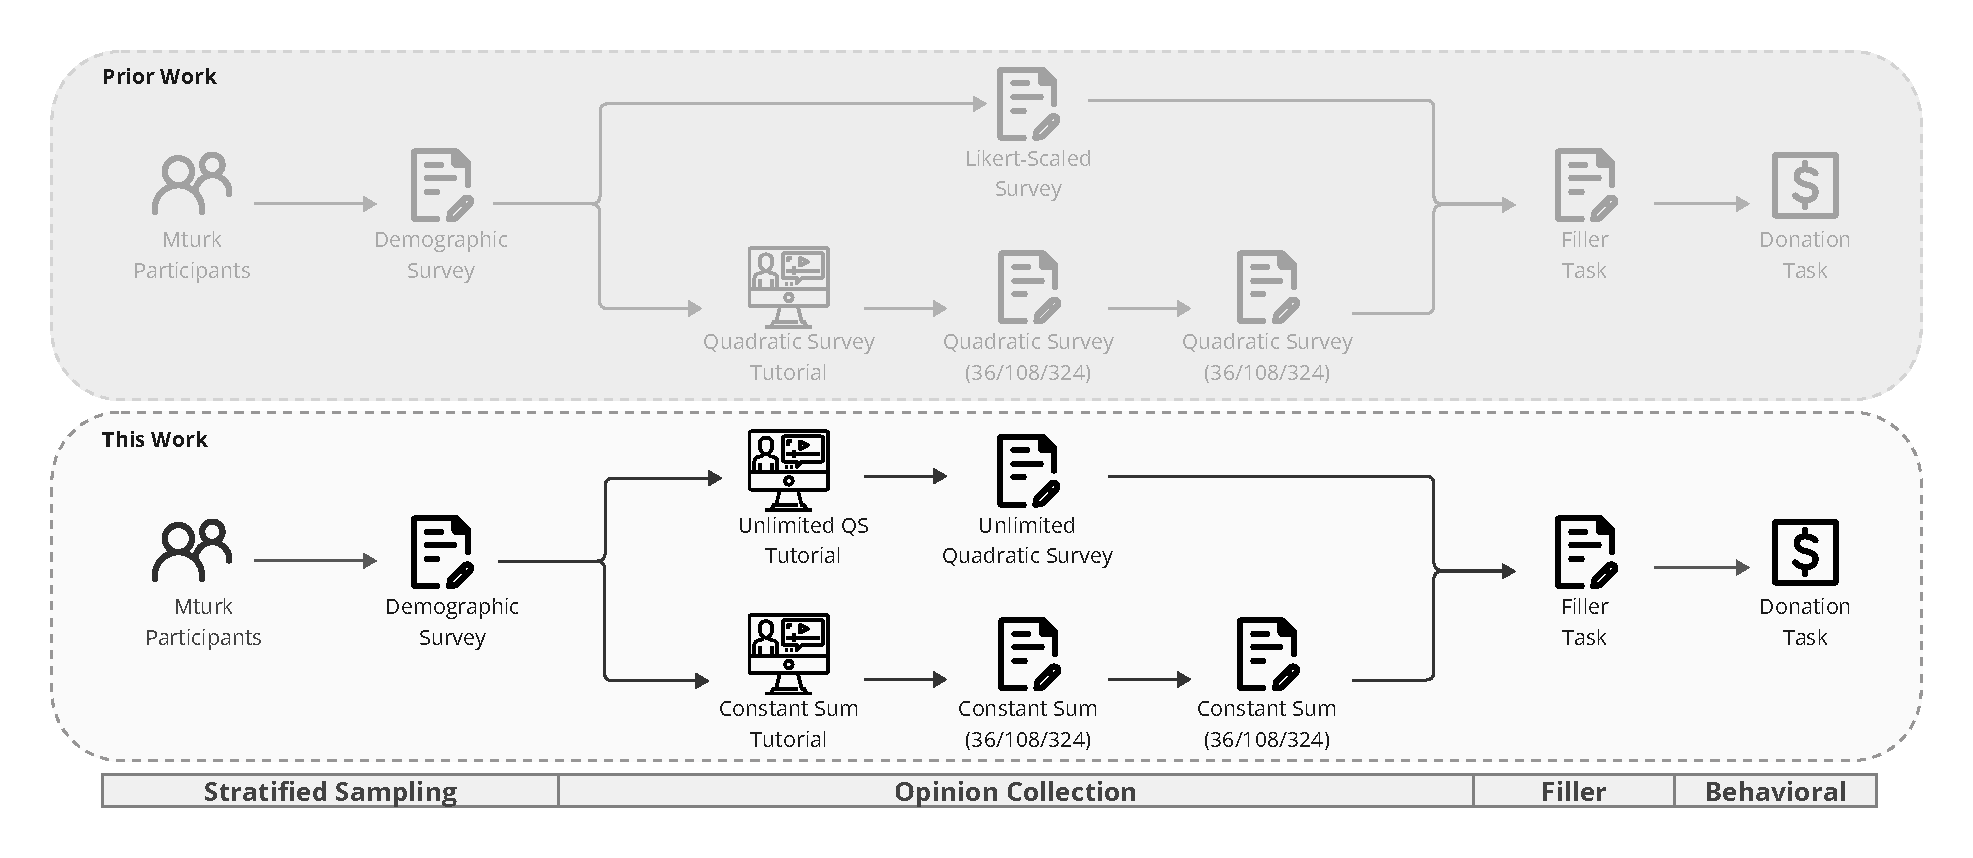
\includegraphics[width=\textwidth]{content/image/whyqs_exp_flow.pdf}
    \caption[]{Experimental design. Our study mirrors the structure of prior work (top,~\cite{chengCanShowWhat2021}), differing only in the opinion collection methods (bottom). This study introduced UQS and LS conditions. The timeline below segments the procedure into four stages, highlighting how our approach mirrors prior work: stratified sampling, opinion collection, filler task, and behavioral task.}
    \label{fig:experiment}
\end{figure*}

\subsection{Study Design Details}
To ensure comparability with prior work~\cite{chengCanShowWhat2021} for subsequent analysis, we retained the original between-subjects design and extended their survey software to implement two additional instruments, yielding four new experimental conditions. The study's survey context and donation task remain unchanged, while the procedural modifications are described in the following subsections. Figure~\ref{fig:experiment} illustrates how this study fits within the broader experimental flow established by prior work.

\paragraph{Additional Experimental Conditions}
We introduced four new experimental conditions, grouped into two categories: UQS and LS. In the UQS condition, we removed the budget constraint to isolate the effect of the quadratic cost function. In the LS conditions, we replaced the quadratic cost function with a linear one and subdivided the design into three budget levels:

\begin{itemize} 
    \item LS18: A small-budget LS with 18 credits
    \item LS54: A medium-budget LS with 54 credits
    \item LS162: A large-budget LS with 162 credits
\end{itemize}

Following prior work, we allocated two credits per option, allowing participants to assign up to $\pm2$, which mirrors the expressive range of a 5-point Likert scale and enables them to express moderate intensity in either direction. With nine options, this corresponds to 18 credits for the LS18 condition. We then scaled the budgets using $O(K)$, $O(K^{1.5})$, and $O(K^2)$ to derive LS18, LS54, and LS162, respectively. For example, $2 \times 9^{1.5} = 54$ is LS54.

\subsubsection{Survey content}
The study frames the survey as a collective decision-making task, where participants express preferences across $9$ societal issues such as education, environment, or health. Participants expressed their degree of preference by assigning positive or negative votes under the UQS or LS mechanism.

\subsubsection{Surveying process and interface}
Participants in both groups were first introduced to the survey and how to use it via a video tutorial. To ensure their understanding of the survey mechanism, participants were asked to complete a quiz with 5 multiple-choice questions. A minimum of three correct answers was required to proceed. We altered the questions based on the survey mechanisms. The interfaces for UQS and LS are shown in~\Cref{fig:extended_interface}.

% create a side by side figure using subfigure

\begin{figure*}
    \centering
    \begin{subfigure}{0.75\textwidth}
        \centering
        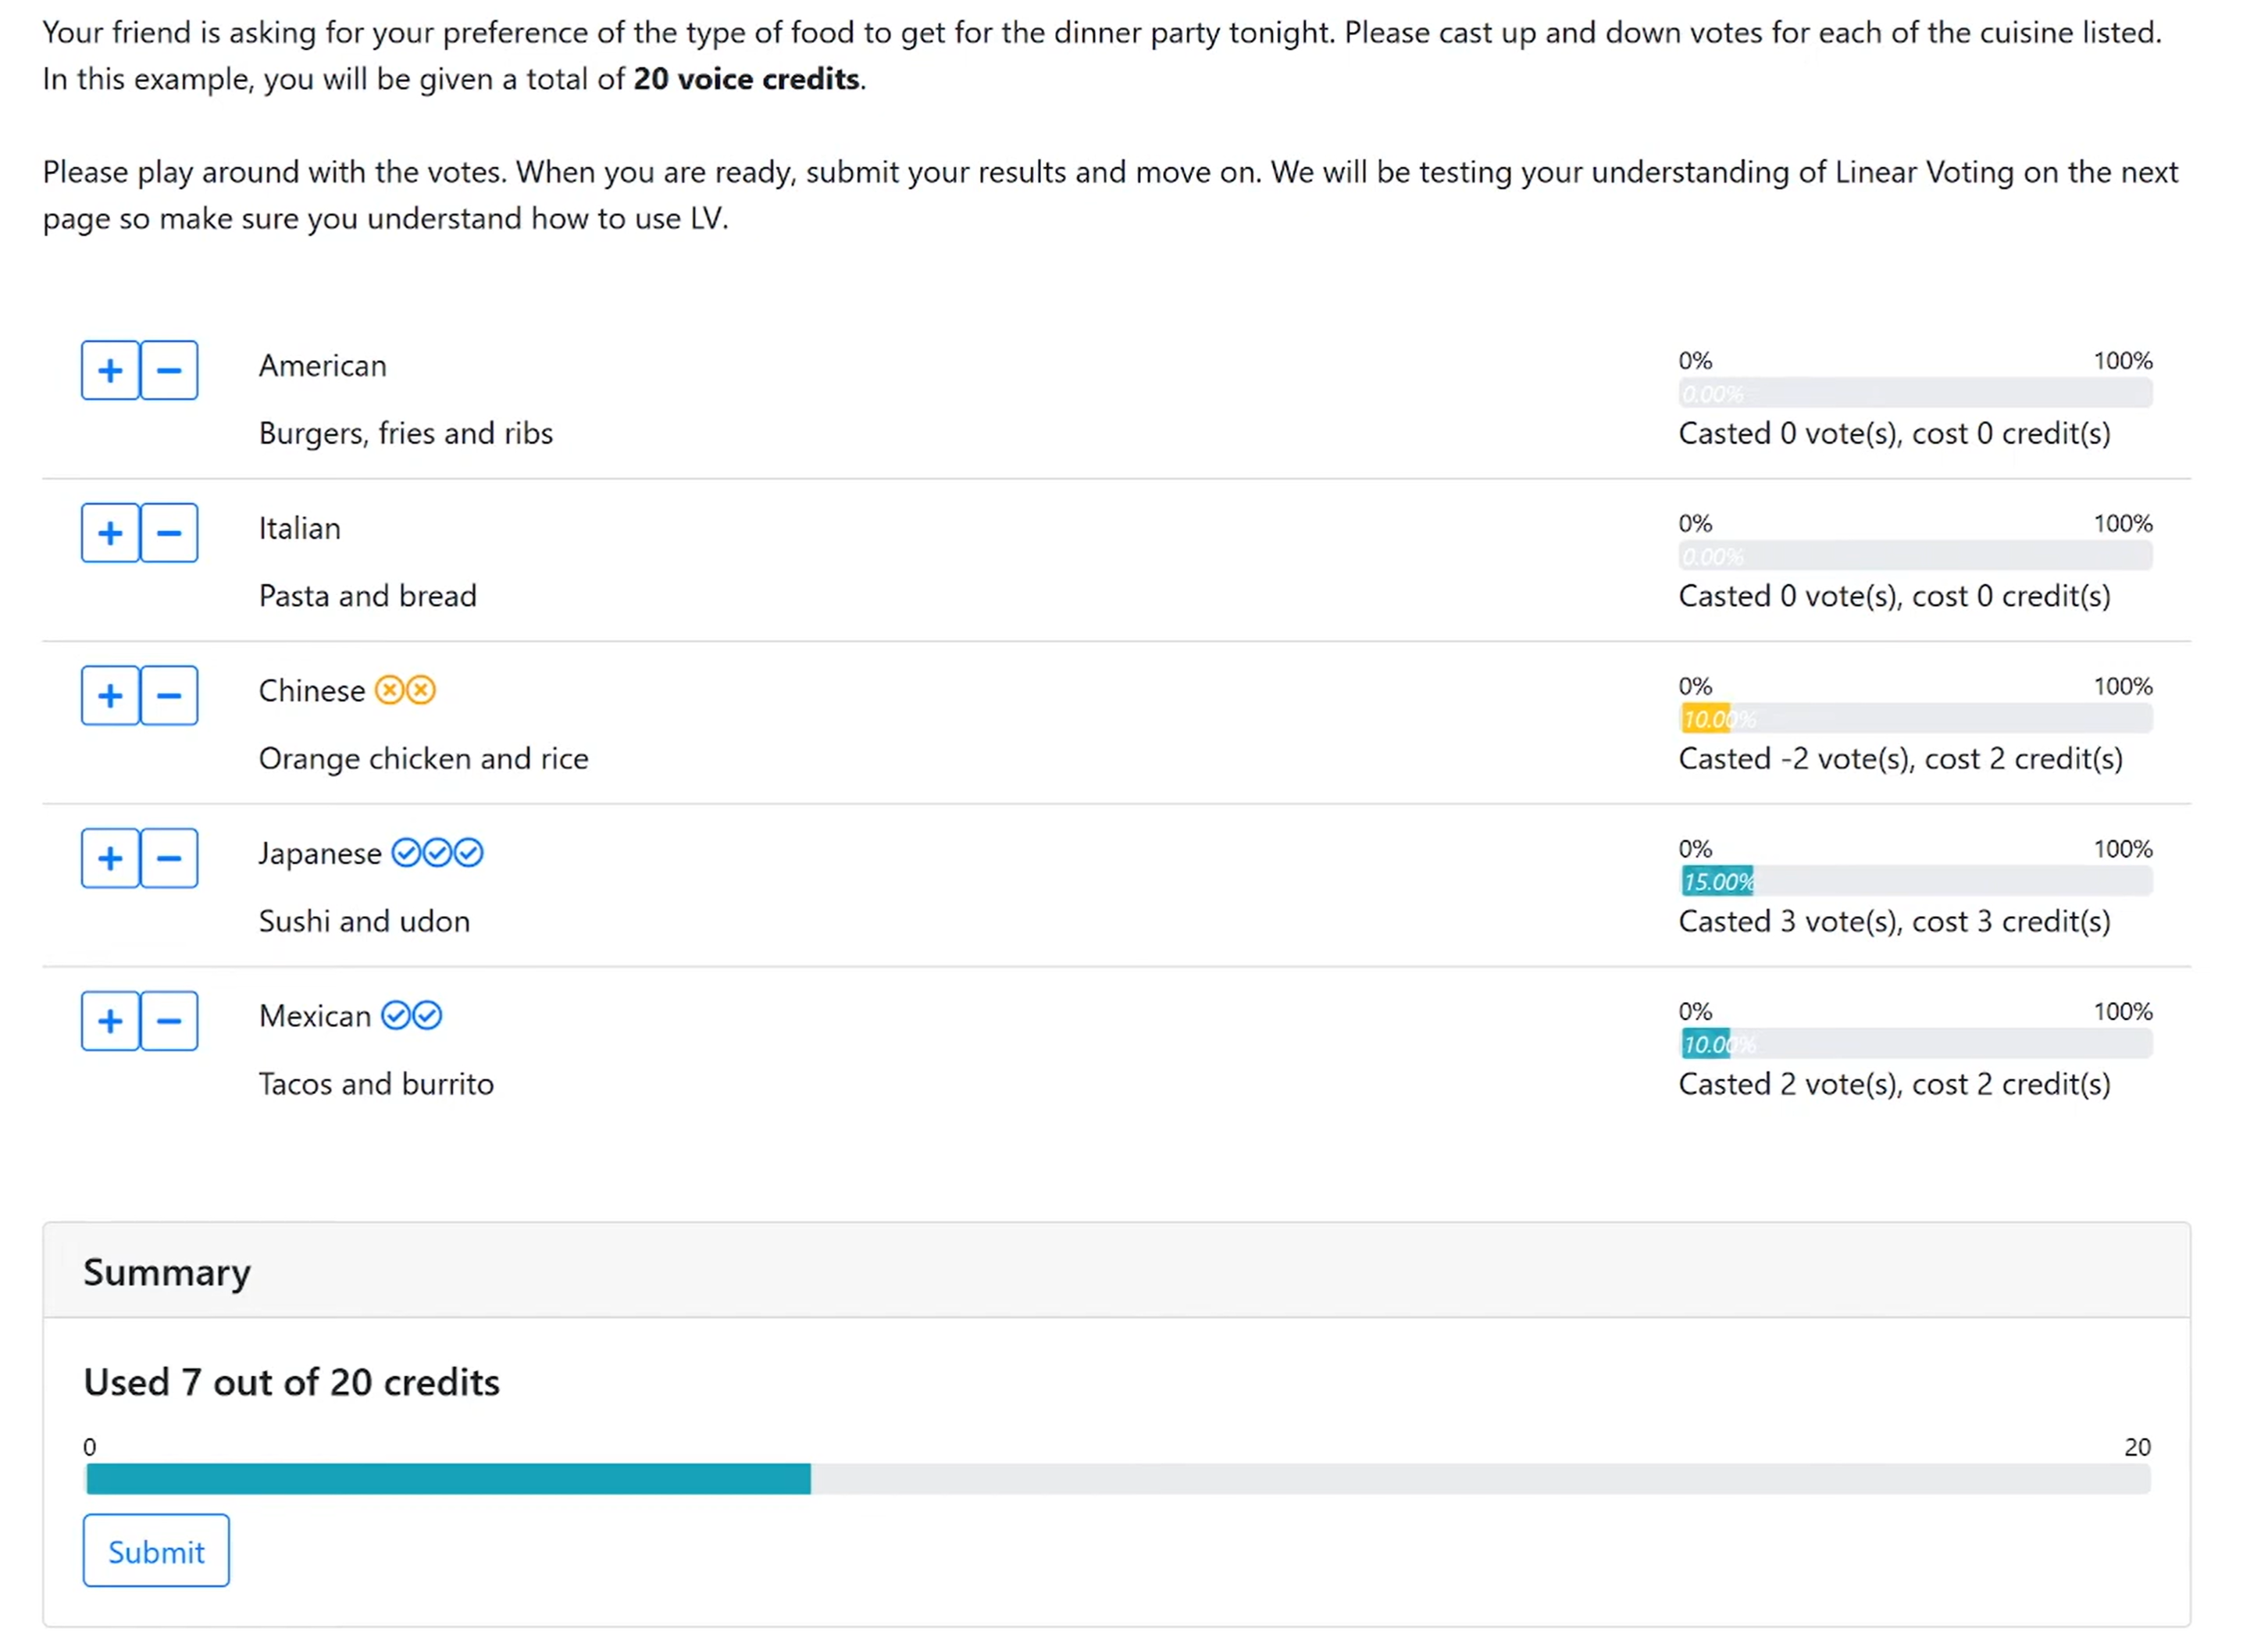
\includegraphics[width=\textwidth]{content/image/linear.png}
        \caption[]{LS Interface: each additional vote is $1$ credit}
        \label{fig:qs_interface}
    \end{subfigure}
    
    \vspace*{1cm}

    \begin{subfigure}{0.75\textwidth}
        \centering
        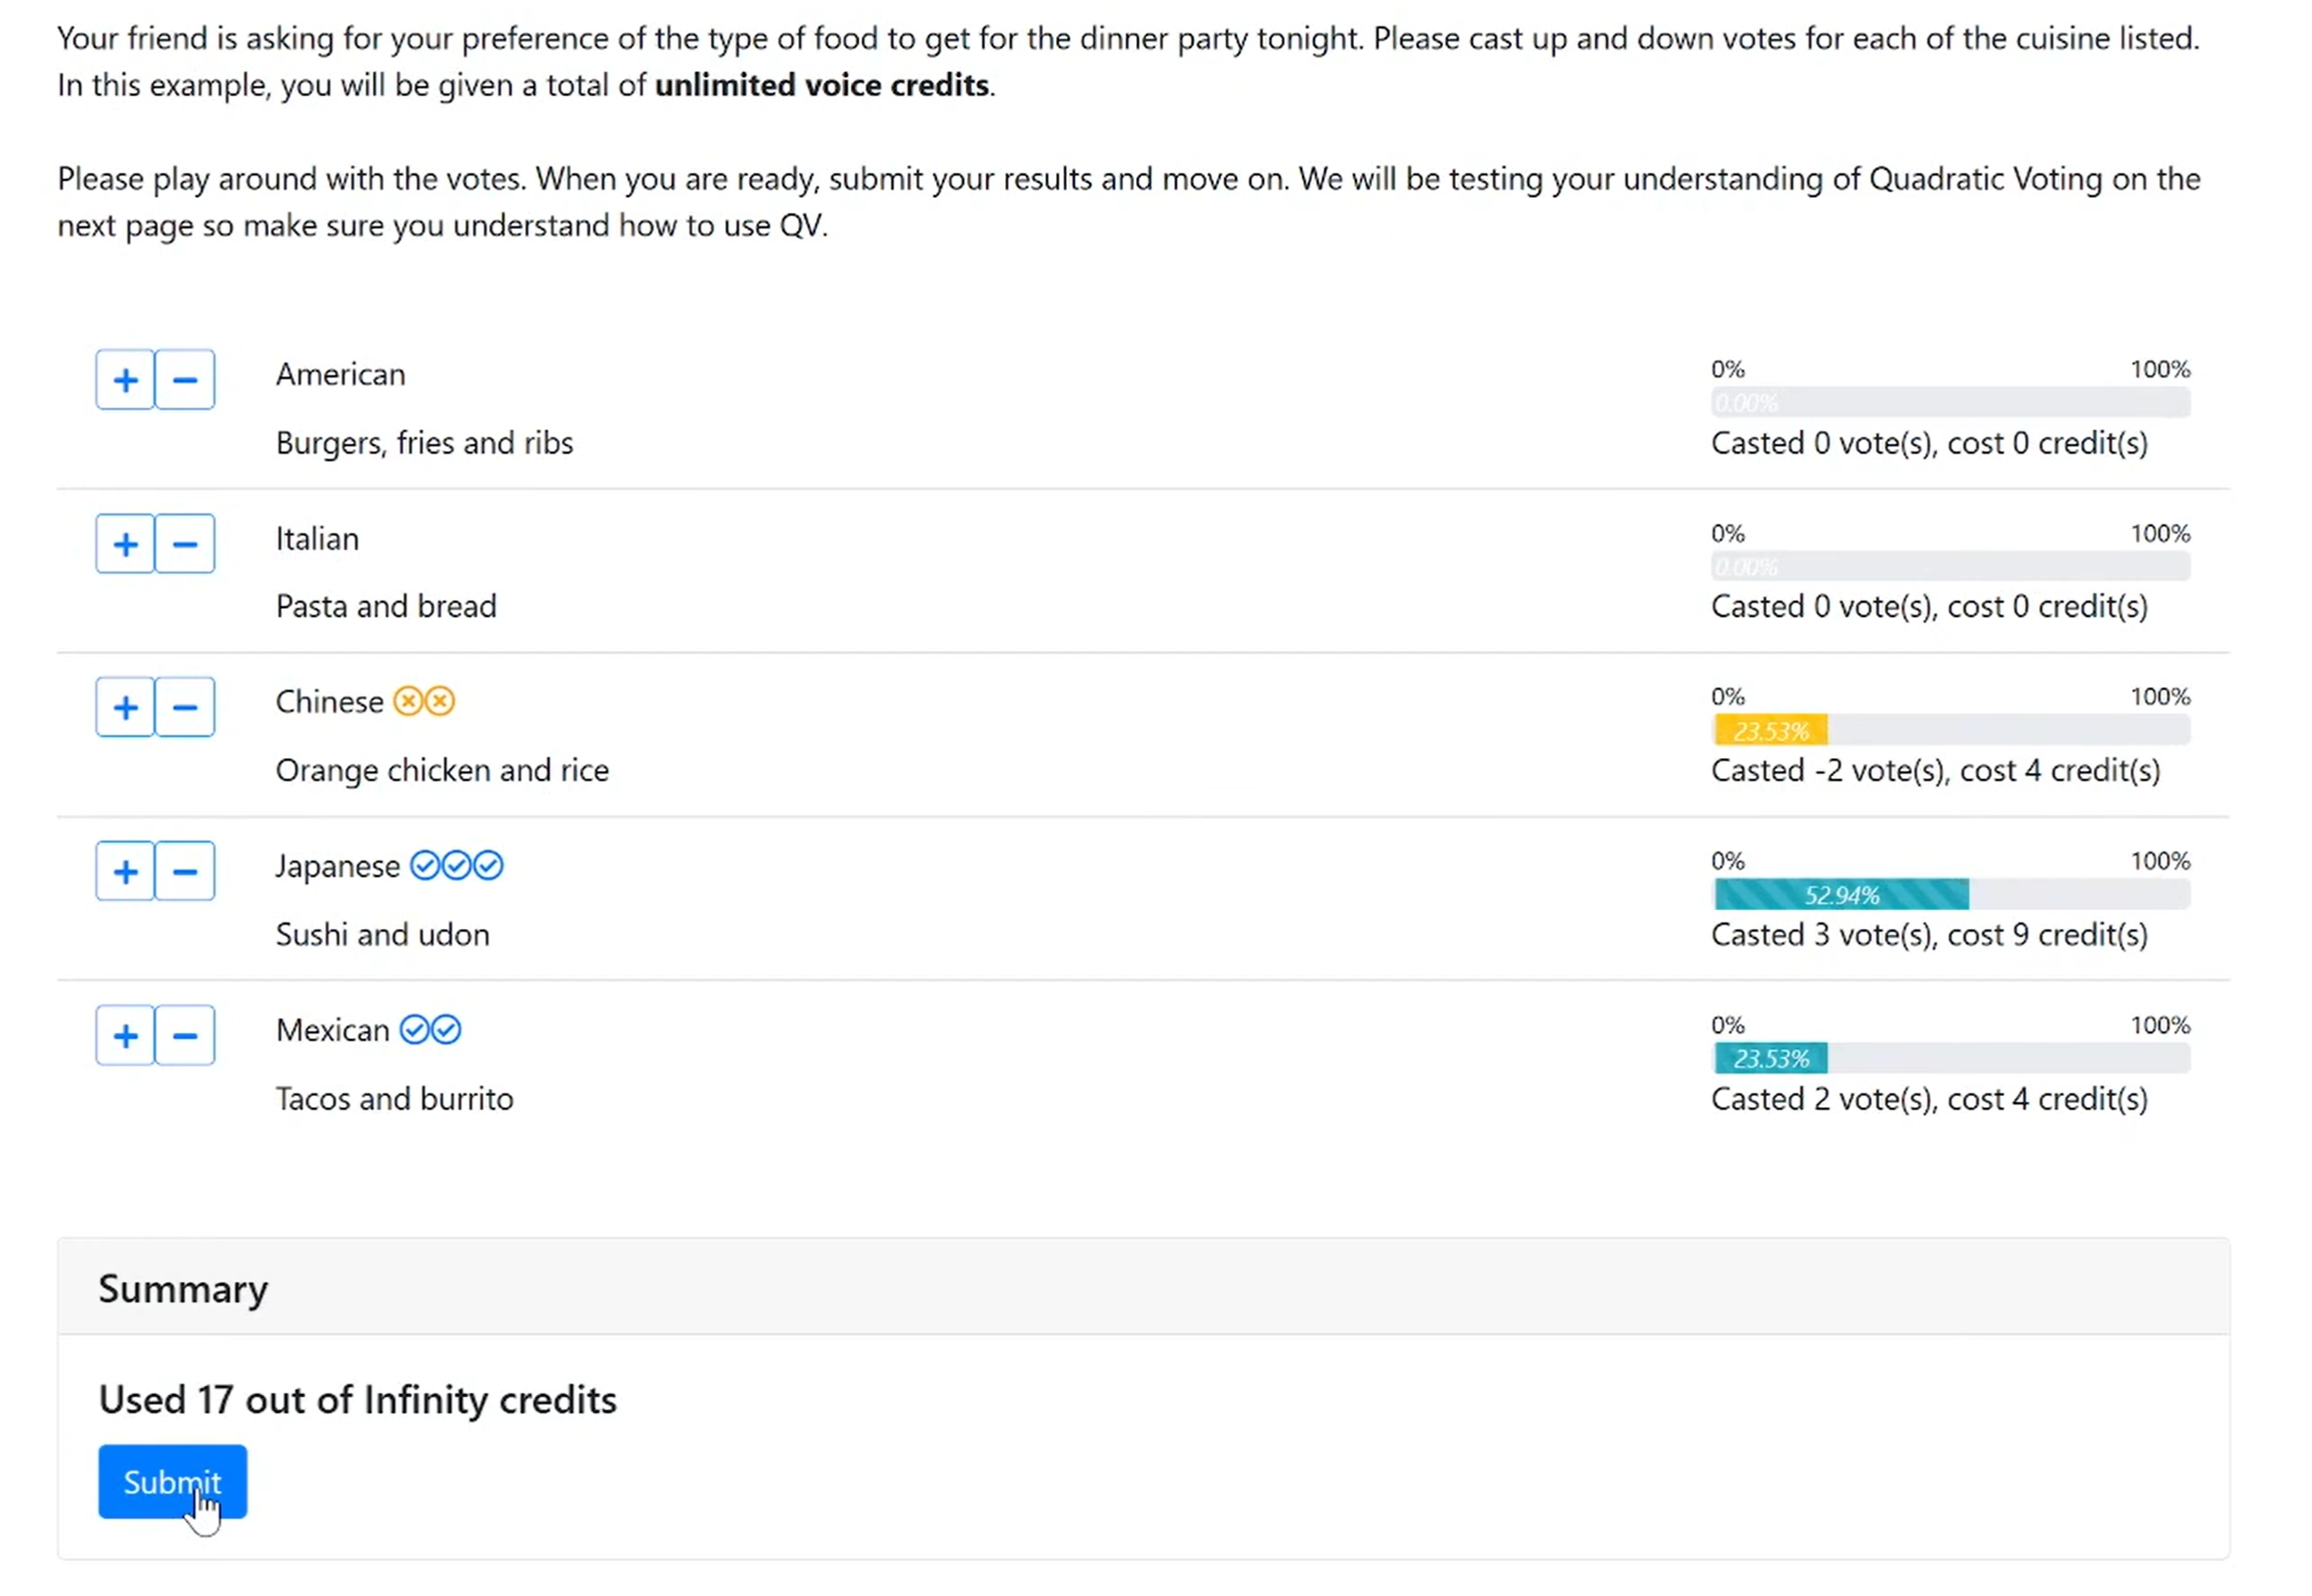
\includegraphics[width=\textwidth]{content/image/uqs.png}
        \caption[]{UQS Interface: each additional vote is $n^2$ credits but does not have a budget constraint}
        \label{fig:css_interface}
    \end{subfigure}
    
    \caption[]{Survey interfaces for the two additional conditions. Each screenshot shows an interactive sandbox that allows  participants to practice the survey mechanism before completing the main task.}
    \label{fig:extended_interface}
\end{figure*}

\subsubsection{Filler task and donation}
After the survey, participants completed a filler task to reduce direct association between survey options and the charities in the donation task. Participants then donated to a set of charities, each representing a distinct cause.

\subsubsection{Debrief and Compensation}
After the study, a debriefing page informed participants of the study’s purpose. Participants were compensated with \$2.50 for their time.

\subsection{Participant Recruitment and Integrating Prior Data}
This study includes both newly collected and publicly available data. We recruited 202 Amazon Mechanical Turk (MTurk) participants using stratified sampling to approximate U.S. census distributions across age, gender, income, and education. Participants were randomly assigned to one of the newly introduced experimental conditions (LS and UQS). This sampling strategy aimed to mitigate demographic imbalances in participation~\cite{redmilesHowWellMy2019}.

We obtained data from previous QS and Likert scale conditions published in~\cite{chengCanShowWhat2021} and included it in this study for comparative evaluation. It covered 219 MTurk participants across two survey types and four experimental conditions: a Likert scale survey and QS with three credit budgets (36, 108, and 324).

To support comparisons across methods, we distinguish between the number of votes assigned to each option (used in the original QS analysis) and the total credits spent per option, which better reflects the cost-based intensity embedded in the quadratic mechanism. We refer to these cost-based representations as QSC36, QSC108, and QSC324.

Altogether, our study evaluates four types of survey instruments: QS, Likert scale survey, LS, and UQS. As summarized in~\Cref{tbl:experiment_cond}, we cover 11 experimental conditions, including three LS budget levels and three QS conditions evaluated using both vote- and cost-based measures. All survey responses were assessed against participant behavior in an incentive-compatible donation task, which serves as a shared behavioral benchmark.

\begin{table*}[h]
    \centering
    \begin{tabular}{@{}lllp{9cm}@{}}
        \toprule
        \textbf{Condition} & \textbf{Budget} & \textbf{Cost Function} & \textbf{Description} \\
        \midrule
        Likert & – & – & A 5-point traditional ordinal-scale survey. \\ 
        \midrule
        Donation & – & – & Incentive-compatible donation task used as behavioral benchmark for validating expressed preferences. \\
        \midrule
        QS36   & 36   & Quadratic & \multirow{3}{9cm}{QS conditions with three different budgets ($O(K)$, $O(K^{1.5})$, $O(K^2)$). Participants expressed preferences by allocating votes, where the cost of each vote increased quadratically, deducted from the budget.} \\
        QS108  & 108  & Quadratic & \\
        QS324  & 324  & Quadratic & \\
        \midrule
        QSC36  & 36   & Quadratic & \multirow{3}{9cm}{Credits that participants contributed per option. Using the results from QS, QSC reflects the actual cost incurred per option to reflect perceived intensity of preference and explore alignment with donation outcomes.} \\
        QSC108 & 108  & Quadratic & \\
        QSC324 & 324  & Quadratic & \\
        \midrule
        LS18   & 18   & Linear    & \multirow{3}{9cm}{Linear-cost versions of QS with budgets scaled as $O(K)$, $O(K^{1.5})$, and $O(K^2)$. Participants expressed preferences by allocating votes, where the cost of each vote increased linearly, deducted from the budget.} \\
        LS54   & 54   & Linear    & \\
        LS162  & 162  & Linear    & \\
        \midrule
        UQS    & Unlimited & Quadratic & QS without a budget where participants expressed preferences by allocating votes, where the cost of each vote increased quadratically, but no budget constraint was enforced. \\
        \midrule
        UQS Credits & Unlimited & Quadratic & Credits participants contributed per option. Using the results from UQS, credits reflect the actual cost incurred per option to reflect perceived intensity of preference and explore alignment with donation outcomes. \\
        \bottomrule
    \end{tabular}
    \caption[]{Overview of survey conditions evaluated in the study, including budget levels, cost structures, and their modeling roles.}
    \label{tbl:experiment_cond}
\end{table*}

%56 completed a Likert scale survey, 107 completed the QS36 survey, 108 completed QS108, and 111 completed QS324.

